%!TEX program = xelatex

\documentclass[a4paper, openany, oneside]{memoir}
\usepackage[no-math]{fontspec}
\usepackage{pgfplots}
\usepackage{float}
\pgfplotsset{compat=newest}
\usepackage{commath}
\usepackage{mathtools}
\usepackage{amssymb}
\usepackage{amsthm}
\usepackage{booktabs}
\usepackage{todonotes}
\usepackage{mathtools}
\usepackage{xcolor}
\usepackage[separate-uncertainty=true, per-mode=symbol]{siunitx}
\usepackage{listings}
\usepackage[american inductor, european resistor]{circuitikz}
\usepackage{amsmath}
\usepackage{amsfonts}
\usepackage{ifxetex}
\usepackage[dutch,english]{babel}
\usepackage[backend=bibtexu,texencoding=utf8,bibencoding=utf8,style=ieee,sortlocale=en_GB,language=auto]{biblatex}
\usepackage[strict,autostyle]{csquotes}
\usepackage{import}
\usepackage{standalone}
\usepackage{bookmark,hyperref}
\usepackage{xcolor,mdframed}
\usepackage{tikz}
\usepackage{framed}
\usepackage{float}
\usepackage{tabularx}
\usepackage{graphicx,adjustbox}
\usepackage{rotating}
\usepackage{pdfpages}
\usepackage{enumitem}
\usepackage{calc}
\usepackage{pgfplots}
\usepackage{filecontents}
\usepackage{caption}
\usepackage{subcaption}
\usepackage{lettrine}

\newcolumntype{Y}{>{\raggedright\arraybackslash}X} % Left-justified text in tabularx environment

\ifxetex{} % Fonts laden in het geval dat je met Xetex compiled
    \usepackage{fontspec}
    \defaultfontfeatures{Scale=MatchLowercase, Ligatures=TeX} % To support LaTeX quoting style
    %\setromanfont{Palatino Linotype} % Tover ergens in Font mapje in root.
    \setsansfont{Avenir Next LT Pro}
    \setromanfont{Adobe Caslon Pro} % Tover ergens in Font mapje in root.
    \setmonofont{Source Code Pro}
\else % Terug val in standaard pdflatex tool chain. Geen ondersteuning voor OTT fonts
    \usepackage[T1]{fontenc}
    \usepackage[utf8]{inputenc}
\fi
\usepackage[noabbrev, capitalize]{cleveref}
\usepackage{ifthen}
\usepackage{titlesec}
\usepackage{titlecaps}

\newcommand{\references}[1]{\begin{flushright}{#1}\end{flushright}}
\renewcommand{\vec}[1]{\boldsymbol{\mathbf{#1}}}
\newcommand{\uvec}[1]{\boldsymbol{\hat{\vec{#1}}}}
\newcommand{\mat}[1]{\boldsymbol{\mathbf{#1}}}
\newcommand{\fasor}[1]{\boldsymbol{\tilde{\vec{#1}}}}
\newcommand{\cmplx}[0]{\mathrm{j}}
\renewcommand{\Re}[0]{\operatorname{Re}}
\newcommand{\Cov}{\operatorname{Cov}}
\newcommand{\Var}{\operatorname{Var}}
\newcommand{\proj}{\operatorname{proj}}
\newcommand{\Perp}{\operatorname{perp}}
\newcommand{\col}{\operatorname{col}}
\newcommand{\rect}{\operatorname{rect}}
\newcommand{\sinc}{\operatorname{sinc}}
\newcommand{\lcm}{\operatorname{lcm}}
%\newcommand{\gcd}{\operatorname{gcd}}
\newcommand{\F}{\mathcal{F}}
\newcommand{\DTFT}{\mathcal{F}_*}
\newcommand{\conj}[1]{#1^*}
\renewcommand{\mod}{\operatorname{mod}}
\newcommand{\rot}{\operatorname{rot}}
\newcommand{\vecsc}[1]{\vec{\textsc{\textbf{#1}}}}
\renewcommand{\ss}[1]{_{#1}}

% Label without linebreak breaker
\newcommand{\lab}[1]{\label{#1}\nolinebreak}

\newtheorem{definition}{Definition}
\newtheorem{theorem}{Theorem}


\DeclareSIUnit{\voltampere}{VA} %apparent power
\DeclareSIUnit{\pii}{\ensuremath{\pi}}

\hypersetup{%setup hyperlinks
    colorlinks,
    citecolor=black,
    filecolor=black,
    linkcolor=black,
    urlcolor=black
}

% Example boxes
\usepackage{fancybox}
\usepackage{framed}
\usepackage{adjustbox}
\newenvironment{simpages}%
{\AtBeginEnvironment{itemize}{\parskip=0pt\parsep=0pt\partopsep=0pt}
\def\FrameCommand{\fboxsep=.5\FrameSep\shadowbox}\MakeFramed{\FrameRestore}}%
{\endMakeFramed}

% Impulse train
\DeclareFontFamily{U}{wncy}{}
\DeclareFontShape{U}{wncy}{m}{n}{<->wncyr10}{}
\DeclareSymbolFont{mcy}{U}{wncy}{m}{n}
\DeclareMathSymbol{\Sha}{\mathord}{mcy}{"58}

\setlength{\parindent}{0pt}
\nonzeroparskip

% Block environment configuration
\newcommand{\BlockLeftMargin}{20pt}
\newcommand{\BlockLeftMarginText}{25pt}
\newcommand{\BlockLeftMarginTextSpacing}{10pt}

% Own colours
\definecolor{gray75}{gray}{0.75}

% Block environment
\newenvironment{block}[3]{%
\makebox{\hspace{-\spinemargin}%
\begin{tikzpicture}[overlay]
    \draw [thick,color=gray75] (\BlockLeftMargin, 0) -- (\paperwidth - \spinemargin, 0);
    \node at (\BlockLeftMarginText, -0.9) [align=left, text width=\spinemargin - \BlockLeftMarginText - \BlockLeftMarginTextSpacing, anchor=west, text depth=1cm] {\textbf{\textsc{#1}}\newline\textit{#3}};
\end{tikzpicture}}%
\nopagebreak\\[0.25em]\ifthenelse{\equal{#2}{}}{}{(\textit{#2}.) }\nopagebreak\nolinebreak}
{\nopagebreak\\[-0.25em]%
\makebox{\hspace{-\spinemargin}%
\begin{tikzpicture}[overlay, remember picture]
    \draw [thick,color=gray75] (\spinemargin,0) -- (\paperwidth - \spinemargin,0);
\end{tikzpicture}} \vspace{0.5em}}

% Theorem
\newcounter{blockTheoremCounter}
\crefname{blockTheoremCounter}{Theorem}{Theorems}
\Crefname{blockTheoremCounter}{Theorem}{Theorems}

\newenvironment{blockTheorem}[1][]{%
\refstepcounter{blockTheoremCounter}%
\begin{block}{theorem \theblockTheoremCounter}{#1}{}}
{\end{block}}

% Definition
\newcounter{blockDefinitionCounter}
\crefname{blockDefinitionCounter}{Definition}{Definitions}
\Crefname{blockDefinitionCounter}{Definition}{Definitions}

\newenvironment{blockDefinition}[1][]{%
\refstepcounter{blockDefinitionCounter}%
\begin{block}{definition \theblockDefinitionCounter}{#1}{}}
{\end{block}}

% Proof
\newcounter{blockProofTheoremCounter}
\crefname{blockProofTheoremCounter}{Proof}{Proofs}
\Crefname{blockProofTheoremCounter}{Proof}{Proofs}

\newenvironment{blockProofTheorem}[1]{%
\refstepcounter{blockProofTheoremCounter}%
\begin{block}{proof of \\ theorem #1}{}{}}
{\qed\end{block}}

% Detail
\newcounter{blockDetailCounter}
\crefname{blockDetailCounter}{Detail}{Details}
\Crefname{blockDetailCounter}{Detail}{Details}

\newenvironment{blockDetail}[1][]{%
\refstepcounter{blockDetailCounter}%
\begin{block}{detail \theblockDetailCounter}{#1}{}}
{\end{block}}

% Redesign chapter headings
\newcommand{\chapternumber}{\thechapter}
\newcommand{\hsp}{\hspace{20pt}}
\titleformat{\chapter}[hang]{\Huge\bfseries}{\chapternumber\hsp\textcolor{gray75}{|}\hsp}{0pt}{\Huge\bfseries}

% Remove headers
% \addtopsmarks{headings}{}{
%   \createmark{chapter}{left}{nonumber}{}{}
% }
% \pagestyle{headings} % Activate changes

% Capitalise headers in a regular way
\renewcommand*{\memUChead}[1]{\titlecap{#1}}

% \hfill for math mode
\newcommand{\pushright}[1]{\intertext{\hfill$\displaystyle #1$}}
\newcommand{\pushline}{\hskip \textwidth minus \textwidth}
\newcommand{\matlab}{\textsc{Matlab}}

\definecolor{code-grey}{HTML}{DDDDDD}
\newcommand{\lib}[1]{\textsf{#1}}
\newcommand{\file}[1]{\textsf{#1}}
\newcommand{\func}[1]{\colorbox{code-grey}{\texttt{#1}}}
\newcommand{\class}[1]{\colorbox{code-grey}{\texttt{#1}}}

% Setup actiepunten
\newenvironment{important}[1][]{%
   \begin{mdframed}[%
      backgroundcolor={red!15}, hidealllines=true,
      skipabove=0.7\baselineskip, skipbelow=0.7\baselineskip,
      splitbottomskip=2pt, splittopskip=4pt, #1]%
   \makebox[0pt]{% ignore the withd of !
      \smash{% ignor the height of !
         \fontsize{32pt}{32pt}\selectfont% make the ! bigger
         \hspace*{-19pt}% move ! to the left
         \raisebox{-2pt}{% move ! up a little
            {\color{red!70!black}\sffamily\bfseries !}% type the bold red !
         }%
      }%
   }%
}{\end{mdframed}}
\newcommand{\excl}[1]{
\begin{important}
  \textbf{#1}
\end{important}
}

\makeatletter
\newcommand\footnoteref[1]{\protected@xdef\@thefnmark{\ref{#1}}\@footnotemark}
\makeatother

% Allow page breaks in display environments
%\allowdisplaybreaks
% S unit for use in Mega Samples per second
\DeclareSIUnit\sample{S}

\newcommand{\CC}{C\nolinebreak\hspace{-.05em}\raisebox{.3ex}{ \textbf{+}}\nolinebreak\hspace{-.10em}\raisebox{.3ex}{\textbf{+}}}
\def\CC{{C\nolinebreak[4]\hspace{-.05em}\raisebox{.3ex}{\textbf{++}}}}


\newcommand{\partauthor}[1]{\gdef\@partauthor{#1}}
\renewcommand{\printparttitle}[1]{
  \parttitlefont #1\\
  \vspace{1.5cm}
  \textnormal{\Large \@partauthor}
}
\addbibresource{../../../../includes/bibliography.bib}

\begin{document}

\section{Coprime sampling}\label{sec:coprime}
This is illustrated in \cref{tkz:coprime_ruler}.

\begin{figure}[H]
\centering
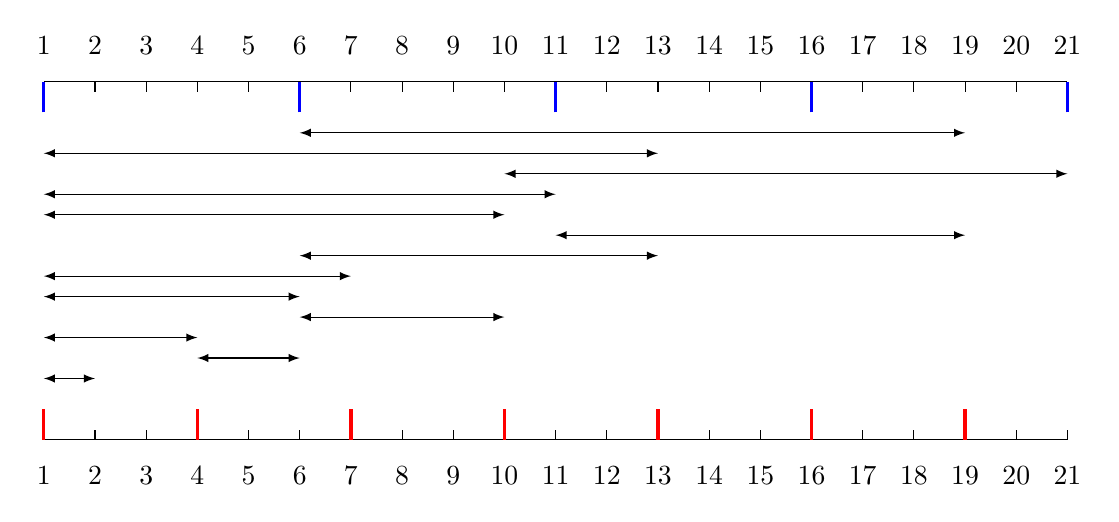
\begin{tikzpicture}[scale=1.3]

\draw (1,0) -- (11,0);

\draw [red, very thick] (1,0) -- (1,0.3);
\draw (1.5,0) -- (1.5,0.1);
\draw (2,0) -- (2,0.1);
\draw [red, very thick] (2.5,0) -- (2.5,0.3);
\draw (3,0) -- (3,0.1);
\draw (3.5,0) -- (3.5,0.1);
\draw [red, very thick] (4,0) -- (4,0.3);
\draw  (4.5,0) -- (4.5,0.1);
\draw (5,0) -- (5,0.1);
\draw [red, very thick] (5.5,0) -- (5.5,0.3);
\draw (6,0) -- (6,0.1);
\draw (6.5,0) -- (6.5,0.1);
\draw [red, very thick] (7,0) -- (7,0.3);
\draw (7.5,0) -- (7.5,0.1);
\draw (8,0) -- (8,0.1);
\draw [red, very thick] (8.5,0) -- (8.5,0.3);
\draw (9,0) -- (9,0.1);
\draw (9.5,0) -- (9.5,0.1);
\draw [red, very thick] (10,0) -- (10,0.3);
\draw (10.5,0) -- (10.5,0.1);
\draw (11,0) -- (11,0.1);

\node at (1,-0.35) {1};
\node at (1.5,-0.35) {2};
\node at (2,-0.35) {3};
\node at (2.5,-0.35) {4};
\node at (3,-0.35) {5};
\node at (3.5,-0.35) {6};
\node at (4,-0.35) {7};
\node at (4.5,-0.35) {8};
\node at (5,-0.35) {9};
\node at (5.5,-0.35) {10};
\node at (6,-0.35) {11};
\node at (6.5,-0.35) {12};
\node at (7,-0.35) {13};
\node at (7.5,-0.35) {14};
\node at (8,-0.35) {15};
\node at (8.5,-0.35) {16};
\node at (9,-0.35) {17};
\node at (9.5,-0.35) {18};
\node at (10,-0.35) {19};
\node at (10.5,-0.35) {20};
\node at (11,-0.35) {21};

\draw (1,3.5) -- (11,3.5);

\draw [blue, very thick] (1,3.2) -- (1,3.5);
\draw (1.5,3.4) -- (1.5,3.5);
\draw (2,3.4) -- (2,3.5);
\draw (2.5,3.4) -- (2.5,3.5);
\draw (3,3.4) -- (3,3.5);
\draw [blue, very thick] (3.5,3.2) -- (3.5,3.5);
\draw (4,3.4) -- (4,3.5);
\draw  (4.5,3.4) -- (4.5,3.5);
\draw (5,3.4) -- (5,3.5);
\draw (5.5,3.4) -- (5.5,3.5);
\draw [blue, very thick] (6,3.2) -- (6,3.5);
\draw (6.5,3.4) -- (6.5,3.5);
\draw (7,3.4) -- (7,3.5);
\draw (7.5,3.4) -- (7.5,3.5);
\draw (8,3.4) -- (8,3.5);
\draw [blue, very thick] (8.5,3.2) -- (8.5,3.5);
\draw (9,3.4) -- (9,3.5);
\draw (9.5,3.4) -- (9.5,3.5);
\draw (10,3.4) -- (10,3.5);
\draw (10.5,3.4) -- (10.5,3.5);
\draw [blue, very thick] (11,3.2) -- (11,3.5);

\node at (1,3.85) {1};
\node at (1.5,3.85) {2};
\node at (2,3.85) {3};
\node at (2.5,3.85) {4};
\node at (3,3.85) {5};
\node at (3.5,3.85) {6};
\node at (4,3.85) {7};
\node at (4.5,3.85) {8};
\node at (5,3.85) {9};
\node at (5.5,3.85) {10};
\node at (6,3.85) {11};
\node at (6.5,3.85) {12};
\node at (7,3.85) {13};
\node at (7.5,3.85) {14};
\node at (8,3.85) {15};
\node at (8.5,3.85) {16};
\node at (9,3.85) {17};
\node at (9.5,3.85) {18};
\node at (10,3.85) {19};
\node at (10.5,3.85) {20};
\node at (11,3.85) {21};

\draw [>=latex,<->] (1,0.6) -- (1.5,0.6);
\draw [>=latex,<->](2.5,0.8) -- (3.5,0.8);
\draw [>=latex,<->](1,1) -- (2.5,1);
\draw [>=latex,<->](3.5,1.2) -- (5.5,1.2);
\draw [>=latex,<->](1,1.4) -- (3.5,1.4);
\draw [>=latex,<->](1,1.6) -- (4,1.6);
\draw [>=latex,<->](3.5,1.8) -- (7,1.8);
\draw [>=latex,<->](6,2) -- (10,2);
\draw [>=latex,<->](1,2.2) -- (5.5,2.2);
\draw [>=latex,<->](1,2.4) -- (6,2.4);
\draw [>=latex,<->](5.5,2.6) -- (11,2.6);
\draw [>=latex,<->](1,2.8) -- (7,2.8);
\draw [>=latex,<->](3.5,3) -- (10,3);

\end{tikzpicture}
\caption{coprime sampling solution with $m=3$ and $n=5$}\label{tkz:coprime_ruler}
\end{figure}

The different sampling periods of the coprime samplers should be chosen carefully. \cite{pal2011coprime} shows that these numbers should be coprime to each other to ensure that all lags are avialable. That means that the sampling periods of the samplers should be $mT$ and $nT$, where the only positive integer that evenly devided both of $m$ and $n$ is 1, hence the name coprime sampling. 

\subsection{Combine coprime sampling with reconstructor}\label{sub:ci-coprime}
The reconstuctor is not designed to process two coprime sampled signals. Therefore some pre-processing is necessary. We need to feed the reconstructor singals of samplers with identical period. To achieve this we break the signals of the two different samplers with sampling period numbers $nT$ and $mT$ into samplers with samopling period $nmT$. This is illustrated in \cref{tkz:pre-coprime}.

\begin{figure}[H]
\centering
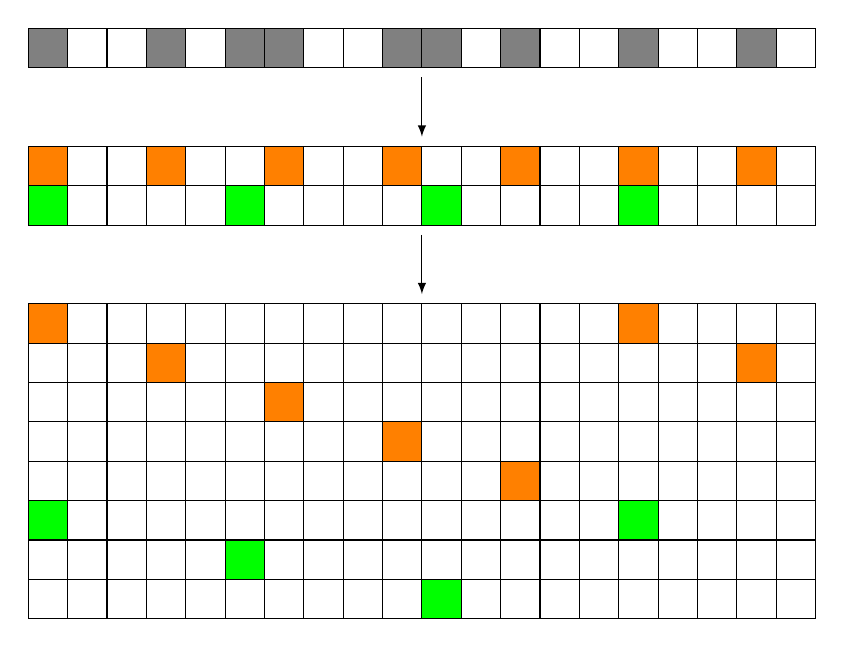
\begin{tikzpicture}
\draw  [fill=gray](-1.5,0.5) rectangle (-1,0);
\draw  (-1,0.5) rectangle (-0.5,0);
\draw  (-0.5,0.5) rectangle (0,0);
\draw  [fill=gray](0,0.5) rectangle (0.5,0);
\draw  (0.5,0.5) rectangle (1,0);
\draw  [fill=gray](1,0.5) rectangle (1.5,0);
\draw  [fill=gray](1.5,0.5) rectangle (2,0);
\draw  (2,0.5) rectangle (2.5,0);
\draw  (2.5,0.5) rectangle (3,0);
\draw  [fill=gray](3,0.5) rectangle (3.5,0);
\draw [fill=gray] (3.5,0.5) rectangle (4,0);
\draw  (4,0.5) rectangle (4.5,0);
\draw  [fill=gray](4.5,0.5) rectangle (5,0);
\draw  (5,0.5) rectangle (5.5,0);
\draw  (5.5,0.5) rectangle (6,0);
\draw [fill=gray](6,0.5) rectangle (6.5,0);
\draw  (6.5,0.5) rectangle (7,0);
\draw  (7,0.5) rectangle (7.5,0);
\draw  [fill=gray](7.5,0.5) rectangle (8,0);
\draw  (8,0.5) rectangle (8.5,0);


\draw  [fill=orange](-1.5,-1) rectangle (-1,-1.5);
\draw  (-1,-1) rectangle (-0.5,-1.5);
\draw  (-0.5,-1) rectangle (0,-1.5);
\draw  [fill=orange](0,-1) rectangle (0.5,-1.5);
\draw  (0.5,-1) rectangle (1,-1.5);
\draw  (1,-1) rectangle (1.5,-1.5);
\draw  [fill=orange](1.5,-1) rectangle (2,-1.5);
\draw  (2,-1) rectangle (2.5,-1.5);
\draw  (2.5,-1) rectangle (3,-1.5);
\draw  [fill=orange](3,-1) rectangle (3.5,-1.5);
\draw  (3.5,-1) rectangle (4,-1.5);
\draw  (4,-1) rectangle (4.5,-1.5);
\draw  [fill=orange](4.5,-1) rectangle (5,-1.5);
\draw  (5,-1) rectangle (5.5,-1.5);
\draw  (5.5,-1) rectangle (6,-1.5);
\draw  [fill=orange](6,-1) rectangle (6.5,-1.5);
\draw  (6.5,-1) rectangle (7,-1.5);
\draw  (7,-1) rectangle (7.5,-1.5);
\draw  [fill=orange](7.5,-1) rectangle (8,-1.5);
\draw  (8,-1) rectangle (8.5,-1.5);
\draw  [fill=green](-1.5,-1.5) rectangle (-1,-2);
\draw  (-1,-1.5) rectangle (-0.5,-2);
\draw  (-0.5,-1.5) rectangle (0,-2);
\draw  (0,-1.5) rectangle (0.5,-2);
\draw  (0.5,-1.5) rectangle (1,-2);
\draw [fill=green] (1,-1.5) rectangle (1.5,-2);
\draw  (1.5,-1.5) rectangle (2,-2);
\draw  (2,-1.5) rectangle (2.5,-2);
\draw  (2.5,-1.5) rectangle (3,-2);
\draw  (3,-1.5) rectangle (3.5,-2);
\draw  [fill=green](3.5,-1.5) rectangle (4,-2);
\draw  (4,-1.5) rectangle (4.5,-2);
\draw  (4.5,-1.5) rectangle (5,-2);
\draw  (5,-1.5) rectangle (5.5,-2);
\draw  (5.5,-1.5) rectangle (6,-2);
\draw [fill=green] (6,-1.5) rectangle (6.5,-2);
\draw  (6.5,-1.5) rectangle (7,-2);
\draw  (7,-1.5) rectangle (7.5,-2);
\draw  (7.5,-1.5) rectangle (8,-2);
\draw  (8,-1.5) rectangle (8.5,-2);


\draw  [fill=orange](-1.5,-3) rectangle (-1,-3.5);
\draw  (-1,-3) rectangle (-0.5,-3.5);
\draw  (-0.5,-3) rectangle (0,-3.5);
\draw  (0,-3) rectangle (0.5,-3.5);
\draw  (0.5,-3) rectangle (1,-3.5);
\draw  (1,-3) rectangle (1.5,-3.5);
\draw  (1.5,-3) rectangle (2,-3.5);
\draw  (2,-3) rectangle (2.5,-3.5);
\draw  (2.5,-3) rectangle (3,-3.5);
\draw  (3,-3) rectangle (3.5,-3.5);
\draw  (3.5,-3) rectangle (4,-3.5);
\draw  (4,-3) rectangle (4.5,-3.5);
\draw  (4.5,-3) rectangle (5,-3.5);
\draw  (5,-3) rectangle (5.5,-3.5);
\draw  (5.5,-3) rectangle (6,-3.5);
\draw  [fill=orange](6,-3) rectangle (6.5,-3.5);
\draw  (6.5,-3) rectangle (7,-3.5);
\draw  (7,-3) rectangle (7.5,-3.5);
\draw  (7.5,-3) rectangle (8,-3.5);
\draw  (8,-3) rectangle (8.5,-3.5);


\draw  (-1.5,-3.5) rectangle (-1,-4);
\draw  (-1,-3.5) rectangle (-0.5,-4);
\draw  (-0.5,-3.5) rectangle (0,-4);
\draw  [fill=orange](0,-3.5) rectangle (0.5,-4);
\draw  (0.5,-3.5) rectangle (1,-4);
\draw  (1,-3.5) rectangle (1.5,-4);
\draw  (1.5,-3.5) rectangle (2,-4);
\draw  (2,-3.5) rectangle (2.5,-4);
\draw  (2.5,-3.5) rectangle (3,-4);
\draw  (3,-3.5) rectangle (3.5,-4);
\draw  (3.5,-3.5) rectangle (4,-4);
\draw  (4,-3.5) rectangle (4.5,-4);
\draw  (4.5,-3.5) rectangle (5,-4);
\draw  (5,-3.5) rectangle (5.5,-4);
\draw  (5.5,-3.5) rectangle (6,-4);
\draw  (6,-3.5) rectangle (6.5,-4);
\draw  (6.5,-3.5) rectangle (7,-4);
\draw  (7,-3.5) rectangle (7.5,-4);
\draw  [fill=orange](7.5,-3.5) rectangle (8,-4);
\draw  (8,-3.5) rectangle (8.5,-4);

\draw  (-1.5,-4) rectangle (-1,-4.5);
\draw  (-1,-4) rectangle (-0.5,-4.5);
\draw  (-0.5,-4) rectangle (0,-4.5);
\draw  (0,-4) rectangle (0.5,-4.5);
\draw  (0.5,-4) rectangle (1,-4.5);
\draw  (1,-4) rectangle (1.5,-4.5);
\draw  [fill=orange](1.5,-4) rectangle (2,-4.5);
\draw  (2,-4) rectangle (2.5,-4.5);
\draw  (2.5,-4) rectangle (3,-4.5);
\draw  (3,-4) rectangle (3.5,-4.5);
\draw  (3.5,-4) rectangle (4,-4.5);
\draw  (4,-4) rectangle (4.5,-4.5);
\draw  (4.5,-4) rectangle (5,-4.5);
\draw  (5,-4) rectangle (5.5,-4.5);
\draw  (5.5,-4) rectangle (6,-4.5);
\draw  (6,-4) rectangle (6.5,-4.5);
\draw  (6.5,-4) rectangle (7,-4.5);
\draw  (7,-4) rectangle (7.5,-4.5);
\draw  (7.5,-4) rectangle (8,-4.5);
\draw  (8,-4) rectangle (8.5,-4.5);


% 
\draw (-1.5,-4.5) rectangle (-1,-5);
\draw  (-1,-4.5) rectangle (-0.5,-5);
\draw  (-0.5,-4.5) rectangle (0,-5);
\draw (0,-4.5) rectangle (0.5,-5);
\draw  (0.5,-4.5) rectangle (1,-5);
\draw  (1,-4.5) rectangle (1.5,-5);
\draw  (1.5,-4.5) rectangle (2,-5);
\draw  (2,-4.5) rectangle (2.5,-5);
\draw  (2.5,-4.5) rectangle (3,-5);
\draw  [fill=orange](3,-4.5) rectangle (3.5,-5);
\draw  (3.5,-4.5) rectangle (4,-5);
\draw  (4,-4.5) rectangle (4.5,-5);
\draw (4.5,-4.5) rectangle (5,-5);
\draw  (5,-4.5) rectangle (5.5,-5);
\draw  (5.5,-4.5) rectangle (6,-5);
\draw  (6,-4.5) rectangle (6.5,-5);
\draw  (6.5,-4.5) rectangle (7,-5);
\draw  (7,-4.5) rectangle (7.5,-5);
\draw  (7.5,-4.5) rectangle (8,-5);
\draw  (8,-4.5) rectangle (8.5,-5);



\draw  (-1.5,-5) rectangle (-1,-5.5);
\draw  (-1,-5) rectangle (-0.5,-5.5);
\draw  (-0.5,-5) rectangle (0,-5.5);
\draw  (0,-5) rectangle (0.5,-5.5);
\draw  (0.5,-5) rectangle (1,-5.5);
\draw  (1,-5) rectangle (1.5,-5.5);
\draw  (1.5,-5) rectangle (2,-5.5);
\draw  (2,-5) rectangle (2.5,-5.5);
\draw  (2.5,-5) rectangle (3,-5.5);
\draw  (3,-5) rectangle (3.5,-5.5);
\draw  (3.5,-5) rectangle (4,-5.5);
\draw  (4,-5) rectangle (4.5,-5.5);
\draw  [fill=orange](4.5,-5) rectangle (5,-5.5);
\draw  (5,-5) rectangle (5.5,-5.5);
\draw  (5.5,-5) rectangle (6,-5.5);
\draw  (6,-5) rectangle (6.5,-5.5);
\draw  (6.5,-5) rectangle (7,-5.5);
\draw  (7,-5) rectangle (7.5,-5.5);
\draw  (7.5,-5) rectangle (8,-5.5);
\draw  (8,-5) rectangle (8.5,-5.5);





\draw  [fill=green](-1.5,-5.5) rectangle (-1,-6);
\draw  (-1,-5.5) rectangle (-0.5,-6);
\draw  (-0.5,-5.5) rectangle (0,-6);
\draw  (0,-5.5) rectangle (0.5,-6);
\draw  (0.5,-5.5) rectangle (1,-6);
\draw  (1,-5.5) rectangle (1.5,-6);
\draw  (1.5,-5.5) rectangle (2,-6);
\draw  (2,-5.5) rectangle (2.5,-6);
\draw  (2.5,-5.5) rectangle (3,-6);
\draw  (3,-5.5) rectangle (3.5,-6);
\draw  (3.5,-5.5) rectangle (4,-6);
\draw  (4,-5.5) rectangle (4.5,-6);
\draw  (4.5,-5.5) rectangle (5,-6);
\draw  (5,-5.5) rectangle (5.5,-6);
\draw  (5.5,-5.5) rectangle (6,-6);
\draw [fill=green] (6,-5.5) rectangle (6.5,-6);
\draw  (6.5,-5.5) rectangle (7,-6);
\draw  (7,-5.5) rectangle (7.5,-6);
\draw  (7.5,-5.5) rectangle (8,-6);
\draw  (8,-5.5) rectangle (8.5,-6);

\draw  (-1.5,-6) rectangle (-1,-6.5);
\draw  (-1,-6) rectangle (-0.5,-6.5);
\draw  (-0.5,-6) rectangle (0,-6.5);
\draw  (0,-6) rectangle (0.5,-6.5);
\draw  (0.5,-6) rectangle (1,-6.5);
\draw [fill=green] (1,-6) rectangle (1.5,-6.5);
\draw  (1.5,-6) rectangle (2,-6.5);
\draw  (2,-6) rectangle (2.5,-6.5);
\draw  (2.5,-6) rectangle (3,-6.5);
\draw  (3,-6) rectangle (3.5,-6.5);
\draw  (3.5,-6) rectangle (4,-6.5);
\draw  (4,-6) rectangle (4.5,-6.5);
\draw  (4.5,-6) rectangle (5,-6.5);
\draw  (5,-6) rectangle (5.5,-6.5);
\draw  (5.5,-6) rectangle (6,-6.5);
\draw  (6,-6) rectangle (6.5,-6.5);
\draw  (6.5,-6) rectangle (7,-6.5);
\draw  (7,-6) rectangle (7.5,-6.5);
\draw  (7.5,-6) rectangle (8,-6.5);
\draw  (8,-6) rectangle (8.5,-6.5);

\draw  (-1.5,-6.5) rectangle (-1,-7);
\draw  (-1,-6.5) rectangle (-0.5,-7);
\draw  (-0.5,-6.5) rectangle (0,-7);
\draw  (0,-6.5) rectangle (0.5,-7);
\draw  (0.5,-6.5) rectangle (1,-7);
\draw  (1,-6.5) rectangle (1.5,-7);
\draw  (1.5,-6.5) rectangle (2,-7);
\draw  (2,-6.5) rectangle (2.5,-7);
\draw  (2.5,-6.5) rectangle (3,-7);
\draw  (3,-6.5) rectangle (3.5,-7);
\draw  [fill=green](3.5,-6.5) rectangle (4,-7);
\draw  (4,-6.5) rectangle (4.5,-7);
\draw  (4.5,-6.5) rectangle (5,-7);
\draw  (5,-6.5) rectangle (5.5,-7);
\draw  (5.5,-6.5) rectangle (6,-7);
\draw  (6,-6.5) rectangle (6.5,-7);
\draw  (6.5,-6.5) rectangle (7,-7);
\draw  (7,-6.5) rectangle (7.5,-7);
\draw  (7.5,-6.5) rectangle (8,-7);
\draw  (8,-6.5) rectangle (8.5,-7);

\node (v1) at (3.5,0) {};
\node (v2) at (3.5,-1) {};
\draw  [>=latex,->](v1) edge (v2);

\node (v3) at (3.5,-2) {};
\node (v4) at (3.5,-3) {};
\draw  [>=latex,->](v3) edge (v4);


\end{tikzpicture}
\caption{pre-proccesing coprime signals}\label{tkz:pre-coprime}
\end{figure}

In this figure, the grey blocks indicate the samples recovered by the device, the orange blocks the samples that are recoverd by sampler $m$, and the green blocks the samples that are recovered by sampler $n$. The middle block shows how the samples are actually gathered, while the bottom block shows how the reconstructor thinks the samples are gathered.

Now that we work with multiple samplers with identical sampling frequency we can use the technique described in \cref{sub:ci-circ} to connect coprime sampling to the reconstructor.
\end{document}
